%%%%%%%%%%%%%%%%%%%%%%%%%%%%%%%%%%%%%%%%%%%%
% 
% Last edits: Nov 9, 2016
%%%%%%%%%%%%%%%%%%%%%%%%%%%%%%%%%%%%%%%%%%%%

\documentclass[12pt]{article}
\usepackage{natbib}
\usepackage[letterpaper, margin=1.1in]{geometry}
\usepackage{graphicx}
\usepackage{wrapfig}
\usepackage{enumitem}
\setlist[enumerate]{itemsep=0mm}
\usepackage{multirow}
\usepackage{lscape}
\usepackage{caption}
\usepackage{subcaption}
\usepackage{hyperref}

\begin{document}
\noindent{Alexandra Pulwicki \\ \today}

\begin{center}
\Large \textbf{Results\\ Observations}
\end{center}


\section*{Overview}

A winter snow survey was conducted on three glaciers in the Donjek Range of the St. Elias Mountains in May 2016. This report documents the field design and planning and how the planned work was implemented in the field.


\pagebreak

%%%%
\section{Field Design}
%%%%

\subsection{Sampling Scheme and Naming System}


\begin{landscape}
\begin{figure}
	\centering
	\fbox{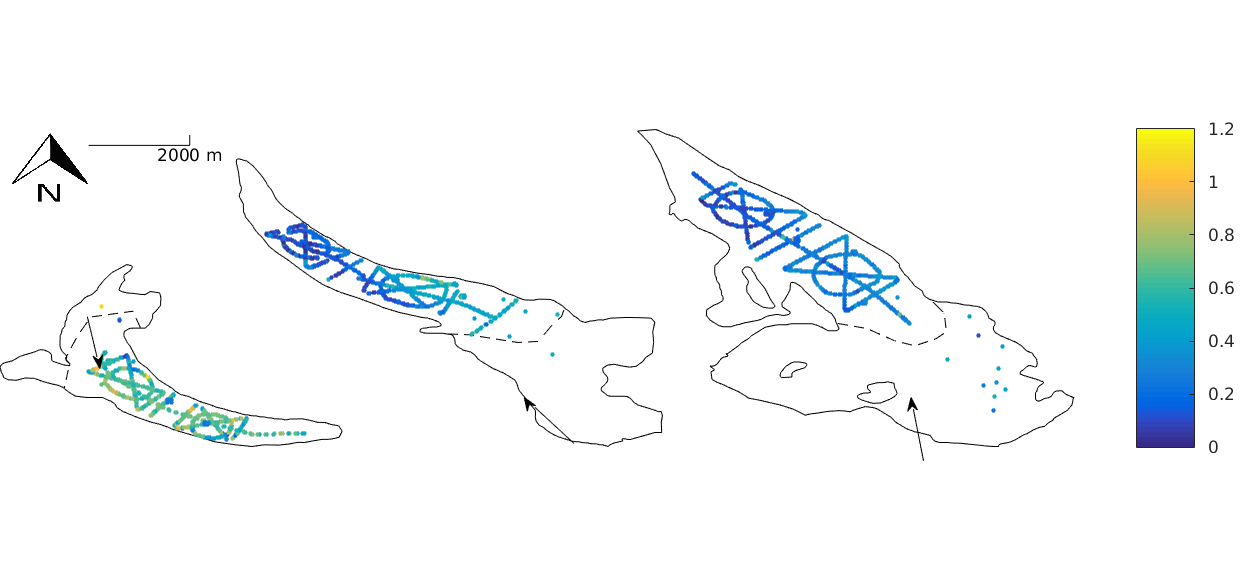
\includegraphics[height = 0.5\textwidth]{SWEmap.png}}\\
	\caption{Estimated snow water equivalent (SWE) at measurement locations. Density was taken to be the average of three integrated, snowpit-derived densities for each glacier.}
	\label{studysites}
\end{figure}


\end{landscape}


 \subsection{Federal Snow Sampler}
\label{sec:SWE}
 
\begin{figure}
    \centering
    \begin{subfigure}[b]{0.38\textwidth}
        \fbox{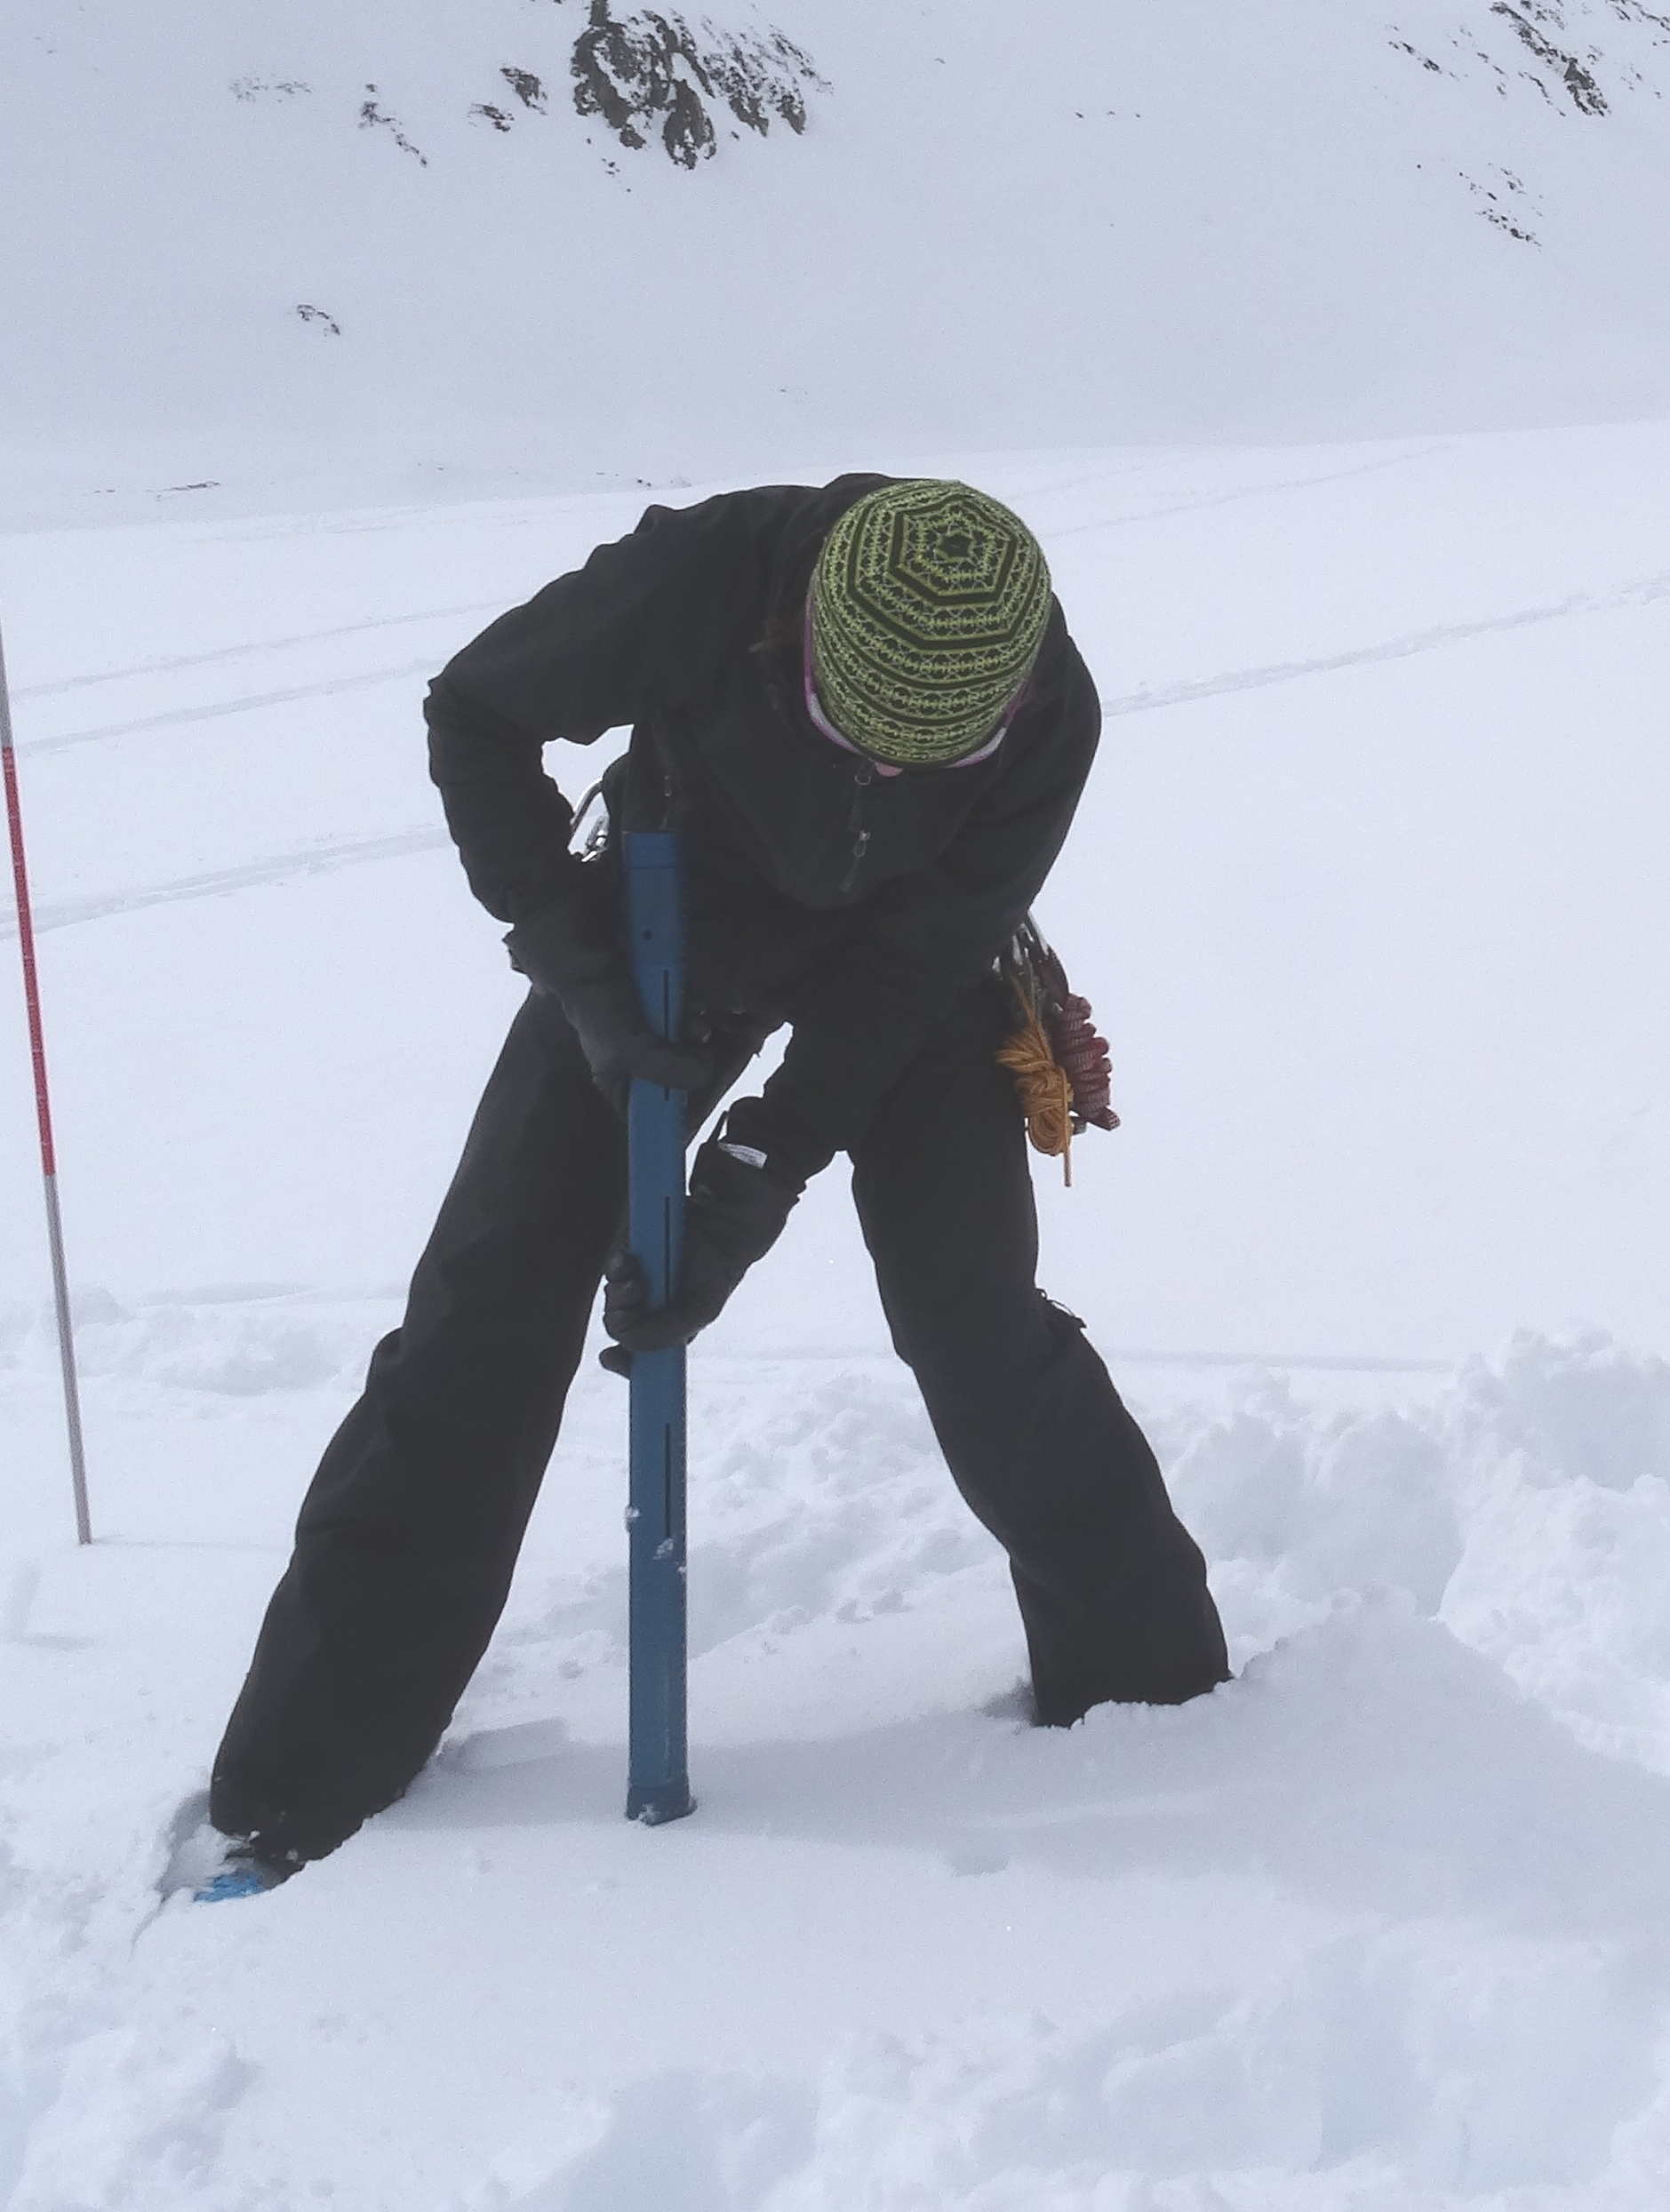
\includegraphics[width=\textwidth]{photo_swe1.JPG}}
        \caption{Inserting the Federal Sampler into the snow. Photo credit: C. Ariagno}
        \label{photo_swe1}
    \end{subfigure}
    ~
    \begin{subfigure}[b]{0.56\textwidth}
        \fbox{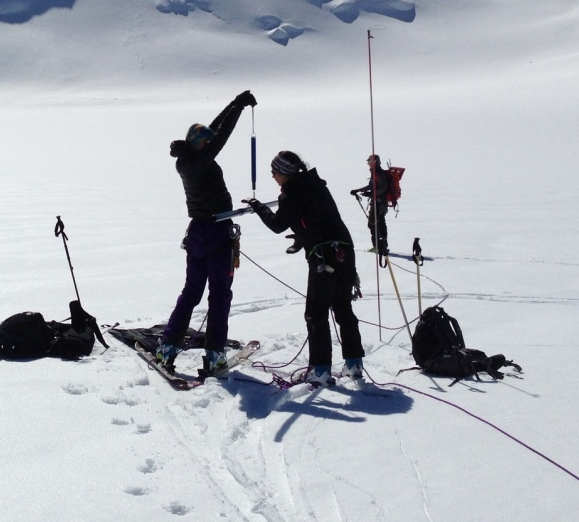
\includegraphics[width=\textwidth]{photo_swe2.jpg}}
        \caption{Weighing the Federal Sampler with snow core on the spring scale (units of cm SWE). Photo credit: G. Flowers}
        \label{photo_swe2}
    \end{subfigure}

    \caption{Using the Federal Sampler to measure SWE}
    \label{photo_swe}
\end{figure}
 
	
%%%%%%%%

\bibliography{/home/glaciology1/Documents/MastersDocuments/MastersLit}
\bibliographystyle{igs}

\end{document}